\chapter{Вмордувинд}
%\corner{64}
\vepsianrose

Как обычно в последний день всеми овладела леность. Осознание того, что пройти осталось совсем немного\mdash расхолаживало. Адмирал, проснувшись, хотел подольше поваляться, но не вышло\mdash погода выдалась на удивление жаркой и солнечной. Яркое утреннее солнце нагрело их с~Замполитом палатку, стало душно. Пришлось вылезать, раскачиваться и варить кофе, который пришёлся как нельзя кстати. День разгорался жаркий и безоблачный\mdash самая что ни на есть днёвочная погодка, а им сегодня сниматься с маршрута. Адмирал чуть не скрежетал зубами из\sdash за этого, пока варил утреннюю кашу. 

Команда тоже вяленько раскачивалась, потихоньку собираясь у костра:

\diagdash Опять овсянка?

\diagdash Завтрак чемпионов, ну!\mdash парировал Адмирал.

\diagdash Нам десяточку сегодня?\mdash спросил Замполит.

\diagdash Угу!\mdash Адмирал попробовал кашу и посолил.

\diagdash Фигня! Даже протеином можно не заряжаться.

\diagdash Фигня\sdash то фигня, но ветер будет, походу, встречный. 

\diagdash О, точно. Тогда протеином всё\sdash таки заряжаться.\mdash Замполит пошёл искать свой бочонок в красной герме$\ldots$

\vspace{0.75em}

$\ldots$На воду ребята встали поздно, около полудня. Как и предсказывал Адмирал, поднялся сильный встречный ветер, вмордувинд. Идти по озеру стало настоящей пыткой. Сверху нещадно палило солнце, они все скинули штормовки, футболки и тельняшки, постоянно смачивали панамы водой\mdash пекло стояло совсем не карельское:

\diagdash Роман Менделич, ну вот вчера бы так!\mdash лопатил Замполит веслом.  

\diagdash Не договорились опять?\mdash Серёга вытащил ноги на~нос байды и грёб полулёжа.

\diagdash Вообще никак, жара!

Адмирал снял тельняшку и повесил её себе на спину, положил GPS\sdash прибор на колени и правил по нему, чтобы не~вилять по курсу на~большой воде, когда нет особых ориентиров:

\diagdash Чёртов вмордувинд! Щас бы двигатель, а не весло!

\diagdash Может Гирвас в другой стороне? И нам под ветер надо?\mdash Замполит тяжело грёб.

\diagdash Да если бы$\ldots$

\vspace{0.75em}
%\vspace{1em}
$\ldots$В борьбе с ветром прошёл где\sdash то час. Маленькая эскадра дошла до середины Викшозера, ширина которого порой достигала одного километра. Параллельно Адмирал старался запримечивать стояночные места на~будущее, но их, как назло, практически не было:

\diagdash Вот если бы не встали позавчера на том мысу и~попёрлись бы в озеро дальше\mdash вот тогда бы точно влипли.

\diagdash Да-а-а, стояночек что\sdash то нема.\mdash Серёга всё грёб полулёжа.

Они прошли средних размеров остров но правому борту:

\diagdash А на острове?\mdash поинтересовался Руслан.

\diagdash Да тоже, гляди, ни пляжиков, ни сходов к воде.\mdash грёб Адмирал.

\diagdash Вода ещё высокая, как мы поняли,\mdash вспомнил Паша,\mdash Вот пляжей и не видно.

\diagdash Может и так$\ldots$

\diagdash Долго нам ещё?\mdash поинтересовалась команда, поскольку ветер стихать даже и не думал.

Адмирал сверился с GPS:

\diagdash Половину только прошли.

\diagdash Да твою ж$\ldots$

\vspace{1em}
$\ldots$Спереди чуть левее по курсу начала нарастать гора. Сверившись с картой, Адмирал понял, что тут должен быть поворот реки и им туда\mdash гора должна была скрыть их от~ветра, по крайней мере Адмирал очень на это надеялся:

\diagdash Вперёд, парни! У этой горы поворачиваем и там на~мысу отдохнём, я выжат как лимон, жара ещё.

\begin{wrapfigure}[15]{l}{0.58\textwidth}
	%\begin{figure}[h]
	\centering
	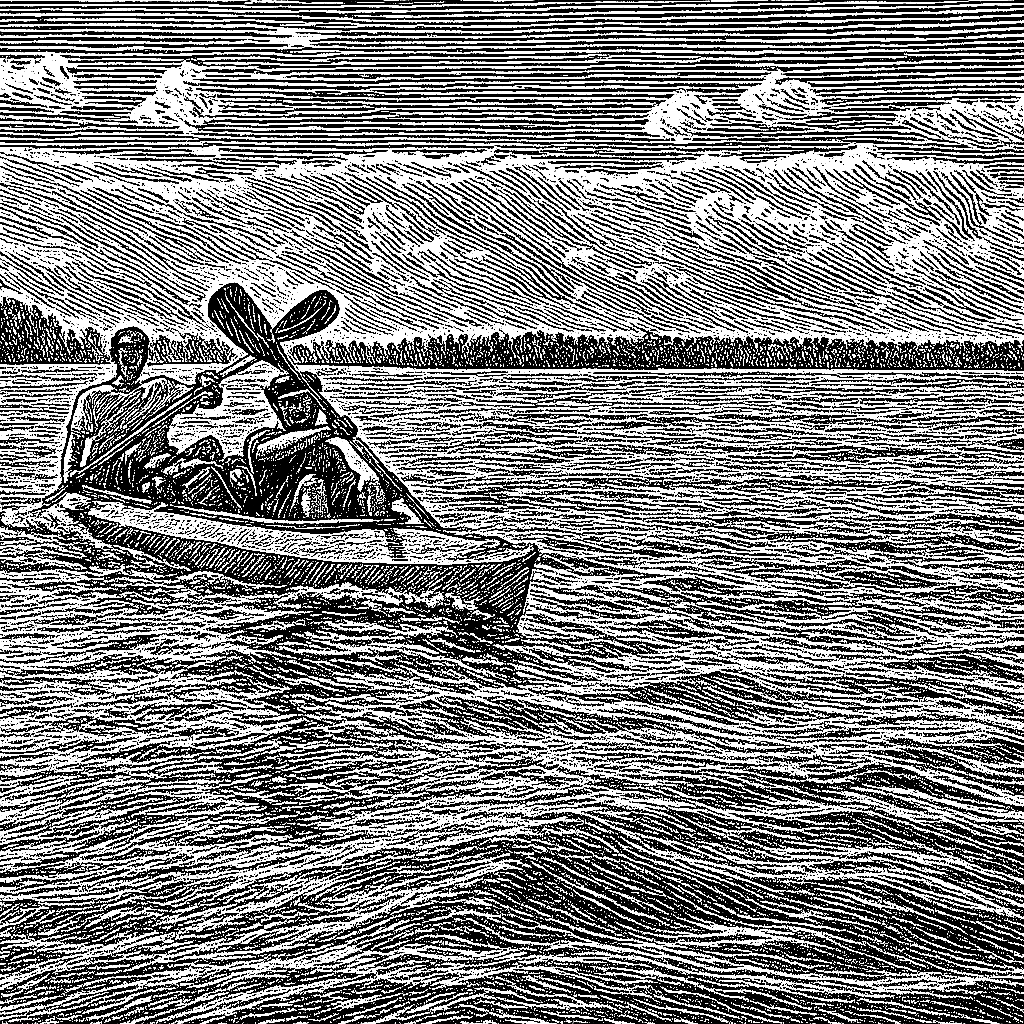
\includegraphics[width=0.57\textwidth]{55_lopatim}
	\caption{\small\textit{...В борьбе с ветром...}}
	%\end{figure}
\end{wrapfigure}
\diagdash Правь давай$\ldots$

Спустя ещё минут 15 они высадились у~истока Суны из~озера на~левом берегу у~хорошей добротной стоянки с~баней. Замполит тут же полез в~вещмешок раздавать всем батончики спортпита подзарядиться:

\diagdash Вот самое моё нелюбимое в Карелии после дождя\mdash это лопатить по озёрам. Особенно против ветра!

\diagdash Полностью согласны!\mdash вздохнули все, запивая батончики чаем из термосов. 

\diagdash Шу-у-урик, гора красивая,\mdash Серёга показал на~правый берег Суны на~ту~самую гору, которая служила ориентиром входа в~реку,\mdash как называется?

Адмирал открыл карту:

\diagdash Никак не называется, по крайней мере официально. Просто высота проставлена и изолинии и больше ничего.

\diagdash Непорядок! Гора Семи Ветров пусть будет!\mdash предложил Замполит, доев батончик.

\diagdash Тебе одного ветра мало было, ты семь захотел? Ы\sdash ы\sdash ы!

\diagdash Ы\sdash ы\sdash ы!\mdash заржали все.

\diagdash Ладно, давайте на воду, тут осталось\sdash то до~Гирваса совсем чуток. Щас по левому берегу пройдём деревню Койкары$\ldots$

$\ldots$Маленькая эскадра правила ближе к левому берегу, ширина русла была около пятисот метров. Деревня была живее всех живых\mdash на берегу купались ребятишки, кто\sdash то полоскал бельё, слышались звуки работы электрорубанков, газонокосилок и других инструментов.

\diagdash Шурик, а впереди развилка?

\diagdash Это островок,\mdash Адмирал сверился с GPS,\mdash обходим его слева, так короче выйдет.

Они обошли остров спустя минут 15, и их взору открылся вид на плотину около Гирваса:

\diagdash А вон и пляжик\mdash последний рывок, парни!\mdash старался приободрить команду Адмирал, сам умирая от~жары.

\diagdash Кто быстрее?\mdash Замполит в своём стиле хотел как всегда потягаться, но у него не вышло\mdash Адмиральская трёшка первой зарылась носом в песок отмели справа от~плотины.

Минуту спустя подтянулся и второй экипаж:

\diagdash Сплав окончен, да здравствует новый Сплав.\mdash провозгласил Адмирал.

\diagdash Шу-у-урик, дальше какие планы?\mdash поинтересовался Серёга.

\diagdash Ну как какие. Разгружаем байды, разбираем каркасы, сушим шкуры, вещи перепаковываем компактнее. \begin{wrapfigure}[18]{l}{0.5\textwidth}
	%\begin{figure}[h]
	\centering
	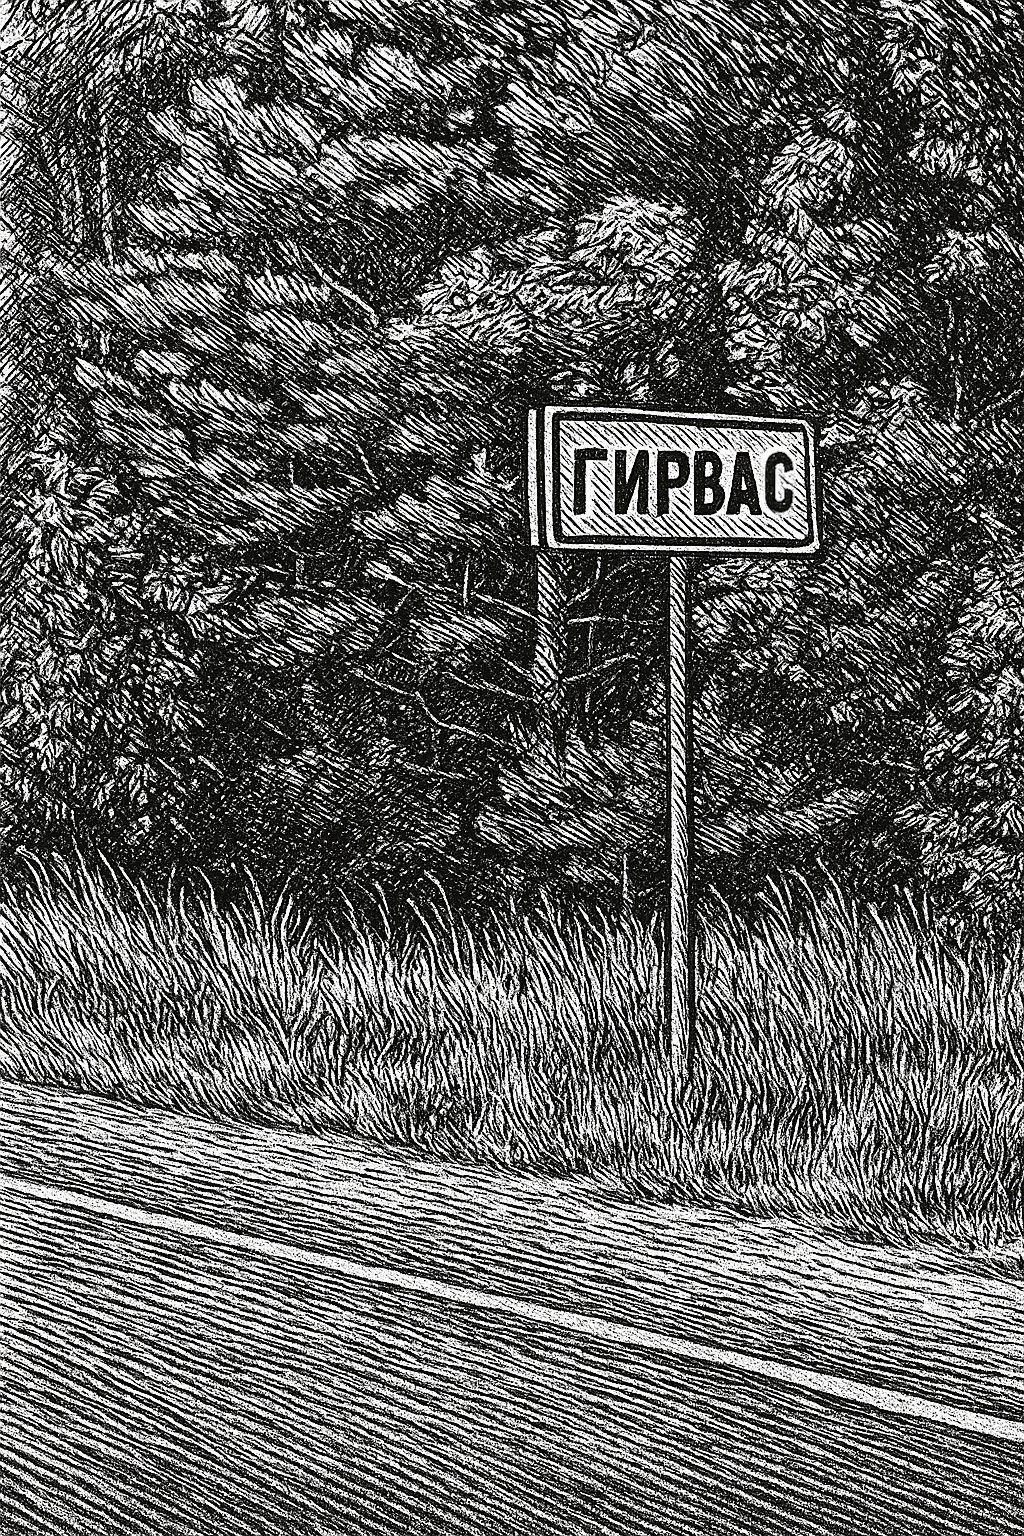
\includegraphics[width=0.48\textwidth]{56_girvas}
	\caption{\small\textit{...пошли~пешком~за~машинами...}}
	%\end{figure}
\end{wrapfigure} Потом мы с тобой пешком смотаемся за~машинами к~Олегу, возвращаемся и всё это загрузим. Как то так$\ldots$

$\ldots$Разборка под палящим солнцем шла еле\sdash еле. Наконец, когда более\sdash менее был достигнут некий порядок, Адмирал решил, что дальше команда справится и без него, и они с Серёгой пошли пешком за~своими авто.

По пути сфоткали указатель <<Гирвас>> и~вскоре после него добрались до двора Олега, где тот встретил их:

\diagdash Ну как отдохнули? Рыбы наловили?

\diagdash Огонь вообще!\mdash эмоции переполняли.\mdash И пороги прошли, и рыбы наловили, щуку даже одну взяли. Короче огонь! Сало ваше ушло на~ура. Словом, всё в наилучшем виде.

\diagdash Рад, рад, ребят. Так что, если что, обращайтесь!\mdash он открыл им ворота, Адмирал с Серёгой выгнали свои машины и, попрощавшись, поехали обратно к берегу.

Вся эта операция отняла прилично времени, потому что пешком было идти довольно далеко, а попутку ловить они не~стали. Пока передовой отряд ходил за авто, остальные успели сгонять в невесть откуда взявшийся местный магазинчик за~пенным и~уже успели изрядно накачаться:

\diagdash Ну вы, блин, даёте!\mdash опешил Адмирал.

\diagdash Ну а фигли вас насухо ждать?

\diagdash Ладно, грузим шмот потихоньку, перетаскивайте все вещмешки к машинам.\mdash распорядился Адмирал и пошёл дозапаковывать свою байду.

Сборы проходили не так чтобы в темпе\mdash пенное быстро развезло вторую часть команды на жаре, но, несмотря на~это, они~справились с~погрузкой. Адмиралу окончательно стало нехорошо от жары, несмотря на то, что он ни капли не выпил:

\diagdash Всё, рассаживайтесь, заедем в магаз купить чё нить на ужин свеженького и в номера, а то я щас просто помру.

\diagdash Всё, маршрут прошли, можешь склеивать ласты, ы\sdash ы\sdash ы!

\diagdash Оч смешно$\ldots$

\vspace{1em}
$\ldots$Вечер парни провели, расслабляясь пенным и~приводя себя в порядок\mdash народ мылся в душе, сбривал бороды, перепаковывал вещи, переодевшись в чистое:

\diagdash Ну вот, можно сказать и всё.\mdash подытожил Замполит.

\diagdash Угу!\mdash Адмирал только к вечеру пришёл в себя после полуденной жары.\mdash Завтра ещё посетим вулкан Гирвас.

\diagdash Вулкан?!

\diagdash Палеовулкан. Он древний и почти разрушенный, там скала такая массивная.\mdash пояснил Адмирал.

\diagdash Кру-у-уто, прико-о-ольно!\mdash одобрила команда.

\diagdash Обратно как стартанём?

\diagdash Шу-у-урик, мы наверно с Русланом через Белозёрск поедем\mdash хочется ещё и его посетить,\mdash заявил Серёга,\mdash ты как, Руслан?

\diagdash Поехали!\mdash подтвердил тот.

\diagdash А мы как, Сань?\mdash спросили Замполит с Пашей.

\diagdash А мы, наверно, до Великого Новгорода? Так более равномерно километраж выйдет на два дня пути?

\diagdash Лад\'{ы}, на том и порешили$\ldots$

$\ldots$Вскоре разговоры стали всё менее оживлёнными, народ утихомирился. Подведение итогов и все пафосные речи остались на их последней стоянке, так что команда, подкошенная усталостью, завалилась спать. Так закольцевалось их озёрно\sdash речное приключение\mdash они вернулись в ту же гостиницу в Гирвасе, из которой стартовали 9 дней назад.

\begin{center}
	\psvectorian[scale=0.4]{88} % Красивый вензелёк :)
\end{center}
